%!TEX root = ../larxxia.tex

\section{Introduction to systems of linear equations}
\label{sec:isle}
\secttoc

\begin{comment}
\pooliv{p.58--64} \layiv{\S1.1} \holti{\S1.1}
\end{comment}


The great aspect of linear equations is that we straightforwardly manipulate them algebraically to deduce results: some results are not only immensely useful in applications but also in further theory.

\begin{example}[simple algebraic manipulation] \label{eg:tempman}
Following \autoref{eg:infertemp}, recall that the temperature in Fahrenheit \(T_F=\frac95T_C+32\) in terms of the temperature in Celsius,~\(T_C\).
Straightforward algebra answers the following questions.
\begin{itemize}
\item What is a formula for the Celsius temperature as a function of the temperature in Fahrenheit?  
Answer by rearranging the equation: subtract~\(32\) from both sides, \(T_F-32=\frac95T_C\)\,;  multiply both sides by~\(\frac59\), then \(\frac59(T_F-32)=T_C\)\,; that is, \(T_C=\frac59T_F-\frac{160}9\)\,.

\item What temperature has the same \emph{numerical value} in the two scales?  
That is, when is \(T_F=T_C\)\,?  
Answer by algebra: we want \(T_C=T_F=\frac95T_C+32\)\,; subtract~\(\frac95T_C\) from both sides to give \(-\frac45T_C=32\)\,; multiply both sides by~\(-\frac54\), then \(T_C=-\frac54\times32=-40\)\,. 
Algebra discovers that~\(-40^\circ\)C is the same temperature as~\(-40^\circ\)F.
\end{itemize}
\end{example}



Linear equations are characterised by each unknown never being multiplied or divided by another unknown, or itself, nor inside `curvaceous' functions.  
\autoref{tbl:linnonlin} lists examples of both.
The power of linear algebra is especially important for large numbers of unknown variables: thousands or millions of variables are common in modern applications.
Generally we say there are \(n\)~unknown variables.
The value of~\(n\) maybe two or three as in many examples, or may be thousands or millions in many modern applications.
\begin{table}
\caption{examples of linear equations, and equations that are not linear (called \idx{nonlinear equation}s).}
\label{tbl:linnonlin}
\begin{equation*}
\begin{array}{l@{\qquad}l}\hline
\text{linear}&\text{nonlinear}\\\hline
-3x+2=0 & x^2-3x+2=0 \\
2x-3y=-1 & 2xy=3\\
-1.2x_1+3.4x_2-x_3=5.6 & x_1^2+2x_2^2=4 \\
r-5s=2-3s+2t & r/s=2+t \\
\sqrt3t_1+\frac\pi2t_2-t_3=0 & 3\sqrt{t_1}+t_2^3/t_3=0\\
(\cos\frac\pi6)x+e^2y=1.23 & x+e^{2y}=1.23\\
\hline
\end{array}
\end{equation*}
\end{table}




\begin{definition} \label{def:lineqn} 
A \bfidx{linear equation} in the \(n\)~variables \(x_1,x_2,\ldots,x_n\) is an equation that can be written in the form
\begin{equation*}
\lincomb axn=b
\end{equation*}
where the \bfidx{coefficient}s \hlist an\ and the \bfidx{constant term}~\(b\) are given scalar constants.
An equation that cannot be written in this form is called a \bfidx{nonlinear equation}.
A \bfidx{system} of linear equations is a set of one or more linear equations in one or more variables (usually more than one).
\end{definition}


\begin{example}[two equations in two variables] \label{eg:2eqs2vars}
Graphically and algebraically solve each of the following systems.
\begin{enumerate}
\item \label{eg:2eqs2vars:a}
\(\begin{array}{l} x+y=3\\2x-4y=0 \end{array}\)
\begin{solution} 
To draw the graphs seen in the marginal plot, rearrange  the linear equations as \(y=3-x\) and \(y=x/2\)\,.  
\marginpar{%
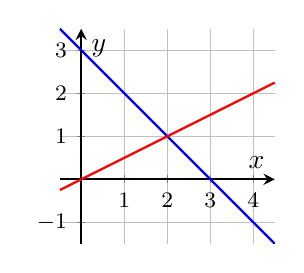
\begin{tikzpicture}[]
\begin{axis}[footnotesize
    , axis equal image, axis lines=middle,
    , xlabel={$x$},ylabel={$y$}, thick, no marks, grid
    , domain=-0.5:4.5 ]
    \addplot{3-x};
    \addplot{x/2};
\end{axis}
\end{tikzpicture}}%
From the graph, they intersect at the point \((2,1)\) so \(x=2\) and \(y=1\) is the unique solution.

Algebraically, one could add twice the first equation to half of the second equation: \(2(x+y)+\frac12(2x-4y)=2\cdot3+\frac12\cdot0\) which simplifies to \(3x=6\) as the \(y\)~terms cancel; hence \(x=2\)\,.  
Then say consider the second equation, \(2x-4y=0\)\,, which now becomes \(2\cdot2-4y=0\)\,, that is, \(y=1\)\,.  
This algebra gives the same solution \((x,y)=(2,1)\) as graphically.
\end{solution}


\item \(\begin{array}{l} 2x-3y=2\\-4x+6y=3 \end{array}\)
\begin{solution} 
To draw the graphs seen in the marginal plot, rearrange  the linear equations as \(y=\frac23x-\frac23\) and \(y=\frac23x+\frac12\)\,.  
\marginpar{%
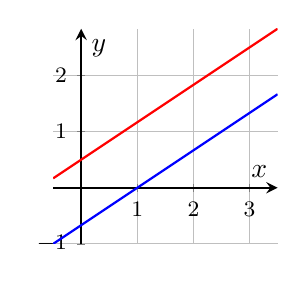
\begin{tikzpicture}[]
\begin{axis}[footnotesize
    , axis equal image, axis lines=middle,
    , xlabel={$x$},ylabel={$y$}, thick, no marks, grid
    , domain=-0.5:3.5 ]
    \addplot{2*x/3-2/3};
    \addplot{2*x/3+1/2};
\end{axis}
\end{tikzpicture}}%
Evidently these lines never intersection, they are parallel, so there appears to be no solution.

Algebraically, one could add twice the first equation to the second equation: \(2(2x-3y)+(-4x+6y)=2\cdot2+3\) which, as the \(x\) and \(y\)~terms cancel, simplifies to \(0=7\)\,. 
This equation is a contradiction as zero is not equal to seven.  
Thus there are no solutions to the system.
\end{solution}

\item \(\begin{array}{l} x+2y=4\\2x+4y=8 \end{array}\)
\begin{solution} 
To draw the graphs seen in the marginal plot, rearrange  the linear equations as \(y=2-x/2\) and \(y=2-x/2\)\,.  
\marginpar{%
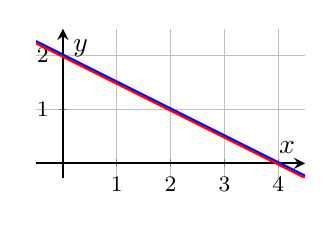
\begin{tikzpicture}[]
\begin{axis}[footnotesize
    , axis equal image, axis lines=middle,
    , xlabel={$x$},ylabel={$y$}, thick, no marks, grid
    , domain=-0.5:4.5, ymax=2.5 ]
    \addplot{2-x/2+0.02};
    \addplot{2-x/2-0.02};
\end{axis}
\end{tikzpicture}}%
They are the same line so every point on this line is a solution of the system.  
There are an infinite number of possible solutions.


Algebraically, the rearrangement of both equations to exactly the same \(y=2-x/2\) establishes an infinite number of solutions, here parametrised by~\(x\).
\end{solution}

\end{enumerate}
\end{example}




\begin{activity}
Solve the system \(x+5y=9\) and \(x+2y=3\) to find the solution is which of the following?
\actposs[4]{\((-1,2)\)}{\((-1,1)\)}{\((1,2)\)}{\((1,1)\)}
%\partswidth=5em
%\begin{parts}
%\item \((-1,1)\)
%\item \((-1,2)\)\actans
%\item \((1,2)\)
%\item \((1,1)\)
%\end{parts}
\end{activity}





\begin{example}[{Global Positioning System}] \label{eg:gps2}
The Global Positioning System (\gps) is a network of 24~satellites orbiting the Earth.
Each satellite knows very accurately its position at all times, and broadcasts this position by radio.
Receivers, such as smart-phones, pick up these signals and from the time taken for the signals to arrive know the distance to those satellites within `sight'.
Each receiver solves a system of equations and informs you of its precise position.

Let's solve a definite example problem, but in two dimensions for simplicity.
Suppose you and your smart-phone are at some unknown location~\((x,y)\) in the 2D-plane, on the Earth's surface where the Earth has radius about \(6\)\,Mm (here all distances are measured in units of Megametres,~Mm, thousands of~km).
But your smart-phone picks up the broadcast from three \gps\ satellites, and then determines their distance from you.
\marginpar{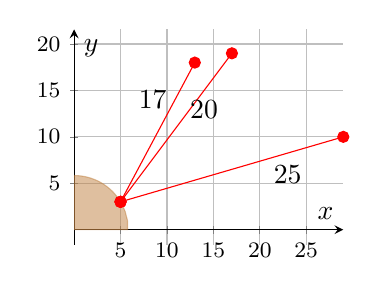
\begin{tikzpicture}[]
\begin{axis}[footnotesize
    , axis equal, axis lines=middle,
    , xlabel={$x$},ylabel={$y$},  grid
    ]
    \addplot[brown,fill,opacity=0.5,domain=0:6]{sqrt(34-x^2)} \closedcycle;
    \addplot[red,mark=*] coordinates {(5,3)(29,10)};
    \node[below] at (axis cs:23,8) {$25$};
    \addplot[red,mark=*] coordinates {(5,3)(17,19)};
    \node[below] at (axis cs:14,15) {$20$};
    \addplot[red,mark=*] coordinates {(5,3)(13,18)};
    \node[left] at (axis cs:11,14) {$17$};
\end{axis}
\end{tikzpicture}}%
From the broadcast and the timing, suppose you then know that a satellite at~\((29,10)\) is \(25\)~away (all in~Mm), one at \((17,19)\) is \(20\)~away, and one at~\((13,18)\) is \(17\)~away (as drawn in the margin).
Find your location~\((x,y)\).


\begin{solution} 
From these three sources of information, Pythagoras and the length of displacement vectors (\autoref{def:veclen}) gives the three equations
\begin{eqnarray*}
&&(x-29)^2+(y-10)^2=25^2\,,
\\&&(x-17)^2+(y-19)^2=20^2\,,
\\&&(x-13)^2+(y-18)^2=17^2\,.
\end{eqnarray*}
These three equations constrain your as yet unknown location~\((x,y)\).
Expanding the squares in these equations gives the equivalent system
\begin{eqnarray*}
&&x^2-58x+841+y^2-20y+100=625\,,
\\&&x^2-34x+289+y^2-38y+361=400\,,
\\&&x^2-26x+169+y^2-36y+324=289\,.
\end{eqnarray*}
Involving squares of the unknowns, \(x^2\)~and~\(y^2\), these are a nonlinear system of equations and so appear to lie outside the remit of this book.  
However, straightforward algebra transforms these three \idx{nonlinear equation}s into a system of two linear equations which we~solve.

Let's subtract the third equation from each of the other two, then the nonlinear squared terms cancel giving a system of two linear equations in two variables:
\begin{eqnarray*}
-32x+672+16y-224=336&\iff&-2x+y=-7\,;
\\-8x+120-2y+37=111&\iff&-4x-y=-23\,.
\end{eqnarray*}%
\marginpar{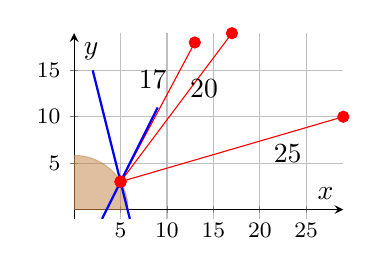
\begin{tikzpicture}[]
\begin{axis}[footnotesize
    , axis equal image, axis lines=middle,
    , xlabel={$x$},ylabel={$y$},  grid
    ]
    \addplot[brown,fill,opacity=0.5,domain=0:6]{sqrt(34-x^2)} \closedcycle;
    \addplot[red,mark=*] coordinates {(5,3)(29,10)};
    \node[below] at (axis cs:23,8) {$25$};
    \addplot[red,mark=*] coordinates {(5,3)(17,19)};
    \node[below] at (axis cs:14,15) {$20$};
    \addplot[red,mark=*] coordinates {(5,3)(13,18)};
    \node[left] at (axis cs:11,14) {$17$};
    \addplot[blue,thick,domain=3:9] {-7+2*x};
    \addplot[blue,thick,domain=2:6] {23-4*x};
\end{axis}
\end{tikzpicture}}%
Graphically, include these two lines to the picture (in blue), namely \(y=-7+2x\) and \(y=23-4x\), and then their intersection gives your location.

Algebraically, one could add the two equations together: \((-2x+y)+(-4x-y)=-7-23\) which reduces to \(-6x=-30\)\,, that is, \(x=5\)\,.
Then either equation, say the first, determines~\(y=-7+2x=-7+2\cdot 5=3\)\,.  
That is, your location is \((x,y)=(5,3)\) (in~Mm), as drawn.
\end{solution}
If the \(x\)-axis is a line through the equator, and the \(y\)-axis goes through the North pole, then trigonometry gives that your location would be at latitude
\(\tan^{-1}\frac35=0.5404=30.96^\circ\)N.
\end{example}





\begin{example}[three equations in three variables] 
\label{eg:3eq3var}
Graph the surfaces and algebraically solve the system
\begin{equation*}
\begin{array}{l}
x_1+x_2-x_3=-2\,,\\
x_1+3x_2+5x_3=8\,,\\
x_1+2x_2+x_3=1\,.
\end{array}
\end{equation*}
\Needspace{4\baselineskip}
\begin{solution} 
The marginal plot shows the three planes represented by the given equations (in the order blue, brown, red), and plots the (black) point we seek of intersection of all three planes.
\marginpar{\begin{tikzpicture}[]
\begin{axis}[footnotesize,height=5cm
, axis equal image, view={55}{35}
, xlabel={$x_1$},ylabel={$x_2$},zlabel={$x_3$},label shift={-1.5ex}
,zmin=1,zmax=3
]
\addplot3[patch,patch type=rectangle,point meta=\thisrow{c}
,opacity=0.6,patch refines=4] table[row sep=\\] {
x y z c \\
0 -2 0 1 \\
0 0 2 1 \\
2 0 4 1 \\
2 -2 2 1 \\
0 -2 2.8 2 \\
0 0 1.6 2 \\
2 0 1.2 2 \\
2 -2 2.4 2 \\
0 0 1 3 \\
0 -1.5 4 3 \\
1 -2 4 3 \\
2 -0.5 0 3 \\
};
\addplot3[only marks,black] coordinates {(1,-1,2)};
\end{axis}
\end{tikzpicture}}

Algebraically we combine and manipulate the equations in a sequence of steps designed to simplify the form of the system.  
\emph{By doing the same manipulation to the whole of each of the equations, we ensure the validity of the result.}
\Needspace{5\baselineskip}
\begin{enumerate}
\item Subtract the first equation from each of the other two equations to deduce (as illustrated)
\marginpar{\begin{tikzpicture}[]
\begin{axis}[footnotesize,height=5cm
,axis equal image, view={55}{35}
, xlabel={$x_1$},ylabel={$x_2$},zlabel={$x_3$},label shift={-1.5ex}
,zmin=1,zmax=3
]
\addplot3[patch,patch type=rectangle,point meta=\thisrow{c}
,opacity=0.6,patch refines=4] table[row sep=\\] {
x y z c \\
0 -2 0 1 \\
0 0 2 1 \\
2 0 4 1 \\
2 -2 2 1 \\
0 0 1.67 2 \\
0 -2 2.33 2 \\
2 -2 2.33 2 \\
2 0 1.67 2 \\
0 0 1.5 3 \\
0 -2 2.5 3 \\
2 -2 2.5 3 \\
2 0 1.5 3 \\
};
\addplot3[only marks,black] coordinates {(1,-1,2)};
\end{axis}
\end{tikzpicture}}
\begin{equation*}
\begin{array}{r@{{}={}}l}
x_1+x_2-x_3&-2\,,\\
2x_2+6x_3&10\,,\\
x_2+2x_3&3\,.
\end{array}
\end{equation*}

\Needspace{5\baselineskip}
\item Divide the second equation by two:
\begin{equation*}
\begin{array}{r@{{}={}}l}
x_1+x_2-x_3&-2\,,\\
x_2+3x_3&5\,,\\
x_2+2x_3&3\,.
\end{array}
\end{equation*}

\Needspace{5\baselineskip}
\item Subtract the second equation from each of the other two (as illustrated):
\marginpar{\begin{tikzpicture}[]
\begin{axis}[footnotesize,height=5cm
,axis equal image, view={55}{35}
, xlabel={$x_1$},ylabel={$x_2$},zlabel={$x_3$},label shift={-1.5ex}
,zmin=1,zmax=3
]
\addplot3[patch,patch type=rectangle,point meta=\thisrow{c}
,opacity=0.6,patch refines=4] table[row sep=\\] {
x y z c \\
0 -2 1.75 1 \\
0 0 1.75 1 \\
2 0 2.25 1 \\
2 -2 2.25 1 \\
0 0 1.67 2 \\
0 -2 2.33 2 \\
2 -2 2.33 2 \\
2 0 1.67 2 \\
0 0 2 3 \\
0 -2 2 3 \\
2 -2 2 3 \\
2 0 2 3 \\
};
\addplot3[only marks,black] coordinates {(1,-1,2)};
\end{axis}
\end{tikzpicture}}
\begin{equation*}
\begin{array}{r@{{}={}}l}
x_1\phantom{+x_2}-4x_3&-7\,,\\
x_2+3x_3&5\,,\\
-x_3&-2\,.
\end{array}
\end{equation*}

\item Multiply the third equation by~\((-1)\):
\begin{equation*}
\begin{array}{r@{{}={}}l}
x_1\phantom{+x_2}-4x_3&-7\,,\\
x_2+3x_3&5\,,\\
x_3&2\,.
\end{array}
\end{equation*}

\Needspace{5\baselineskip}
\item Add four times the third equation to the first, and subtract three times it from the second (as illustrated):
\marginpar{\begin{tikzpicture}[]
\begin{axis}[footnotesize,height=5cm
,axis equal image, view={55}{35}
, xlabel={$x_1$},ylabel={$x_2$},zlabel={$x_3$},label shift={-1.5ex}
,zmin=1,zmax=3
]
\addplot3[patch,patch type=rectangle,point meta=\thisrow{c}
,opacity=0.6,patch refines=4] table[row sep=\\] {
x y z c \\
1 -2 1 1 \\
1  0 1 1 \\
1  0 3 1 \\
1 -2 3 1 \\
0 -1 1 2 \\
0 -1 3 2 \\
2 -1 3 2 \\
2 -1 1 2 \\
0  0 2 3 \\
0 -2 2 3 \\
2 -2 2 3 \\
2  0 2 3 \\
};
\addplot3[only marks,black] coordinates {(1,-1,2)};
\end{axis}
\end{tikzpicture}}%
\begin{equation*}
\begin{array}{r@{{}={}}l}
x_1\phantom{+x_2-4x_3}&1\,,\\
x_2\phantom{+3x_3}&-1\,,\\
x_3&2\,.
\end{array}
\end{equation*}
\end{enumerate}
Thus the only solution to this system of three linear equations in three variables is \((x_1,x_2,x_3)=(1,-1,2)\)\,.
\end{solution}
\end{example}

The sequence of marginal graphs in the previous \autoref{eg:3eq3var} illustrate the equations at each main step in the algebraic manipulations.  
Apart from keeping the solution point fixed, the sequence of graphs looks rather chaotic.
Indeed there is no particular geometric pattern or interpretation of the steps in this algebra.
One feature of \autoref{sec:fisvd} is that we discover how the so-called `singular value decomposition' solves linear equations via a great method with a strong geometric interpretation.
This geometric interpretation then empowers further methods useful in applications.



\paragraph{Transform into abstract setting}
Linear algebra has an important aspect crucial in applications.
A crucial skill in applying linear algebra is that it takes an application problem and transforms it into an abstract setting.
\autoref{eg:infertemp} transformed the problem of inferring a line through two data points into solving two linear equations.
The next \autoref{eg:inf3pts} similarly transforms the problem of inferring a plane through three data points into solving three linear equations.
The original application is often not easily recognisable in the abstract version. 
Nonetheless, it is the abstraction by linear algebra that empowers immense results.


\begin{example}[infer a surface through three points] \label{eg:inf3pts}
This example illustrates the previous paragraph.
Given a geometric problem of inferring what plane passes through three given points, we transform this problem into the linear algebra task of finding the intersection point of three specific planes.
This task we do.

%\begin{comment}
%Could make more realistic application, and more `spread out' data on surface.
%\end{comment}

Suppose we observe that at some given temperature and humidity we get some rainfall: let's find a formula that predicts the rainfall from temperature and humidity measurements.
In some \emph{completely artificial units}, \autoref{tbl:thr} lists measured temperature (`temp'), humidity (`humid'), and rainfall (`rain').
\begin{table}
\caption{in some artificial units, this table lists measured temperature, humidity, and rainfall.}
\label{tbl:thr}
\begin{equation*}
\begin{array}{rrr} \hline
\text{`temp'}&\text{`humid'}&\text{`rain'}\\\hline
1&-1&-2\\
3&5&8\\
2&1&1\\\hline
\end{array}
\end{equation*}
\end{table}

\marginpar{%
\begin{tikzpicture}[]
\begin{axis}[footnotesize,font=\footnotesize,width=\marginparwidth
    , xlabel={temp},ylabel={humid},zlabel={rain},label shift={-1.5ex}
    , domain=-1:5, samples=2
    ]
    \addplot3+[only marks] coordinates {(1,-1,-2)(3,5,8)(2,1,1)};
    \addplot3[surf,opacity=0.5,red] {1-x+2*y};
\end{axis}
\end{tikzpicture}
}
\begin{solution} 
To infer a relation to hold generally---to fill in the gaps between the known measurements, seek `rainfall' to be predicted by the linear formula
\begin{equation*}
\text{(`rain')}=x_1+x_2\text{(`temp')}+x_3\text{(`humid')},
\end{equation*}
for some coefficients~\(x_1\), \(x_2\) and~\(x_3\) to be determined.
The measured data of \autoref{tbl:thr} constrains and determines these coefficients:
substitute each triple of measurements to require
\begin{equation*}
\begin{array}{l}
-2=x_1+x_2(1)+x_3(-1),
\\ 8=x_1+x_2(3)+x_3(5),
\\1=x_1+x_2(2)+x_3(1),
\end{array}
\iff
\begin{array}{l}
x_1+x_2-x_3=-2,
\\ x_1+3x_2+5x_3=8,
\\x_1+2x_2+x_3=1.
\end{array}
\end{equation*}
The previous \autoref{eg:3eq3var} solves this set of three linear equations in three unknowns to determine the solution that the coefficients \((x_1,x_2,x_3)=(1,-1,2)\).
That is, the requisite formula to infer rain from any given temperature and humidity is 
\begin{equation*}
\text{(`rain')}=1-\text{(`temp')}+2\text{(`humid')}.
\end{equation*}

This example illustrates that the geometry of fitting a plane to three points (as plotted) translates into the abstract geometry of finding the intersection of three planes (plotted in the previous example).
The linear algebra procedure for this latter abstract problem then gives the required `physical' solution.
\end{solution}
\end{example}


\begin{figure}
\def\wid{18em}
\centering
\begin{tabular}{@{}cc@{}}
(a)
\begin{tikzpicture}[]
\begin{axis}[footnotesize,width=\wid
, axis equal image
, xlabel={$x_1$},ylabel={$x_2$},zlabel={$x_3$},label shift={-1.5ex}
]
\addplot3[patch,patch type=rectangle,point meta=\thisrow{c}
,opacity=0.6,patch refines=3] table {
x y z c
0 0 2 1
0 5 2 1
5 5 1 1
5 0 1 1
0 2 0 2
0 3 4 2
5 3 4 2
5 2 0 2
2 0 0 3
2 5 0 3
1 5 4 3
1 0 4 3
};
\addplot3[only marks,black] coordinates {(1.58,2.42,1.68)};
\end{axis}
\end{tikzpicture}
& (b)
\begin{tikzpicture}[]
\begin{axis}[footnotesize,width=\wid
, axis equal image
, xlabel={$x_1$},ylabel={$x_2$},zlabel={$x_3$},label shift={-1.5ex}
]
\addplot3[patch,patch type=rectangle,point meta=\thisrow{c}
,opacity=0.6,patch refines=3] table {
x y z c
0 0 2 1
0 5 2 1
5 5 1 1
5 0 1 1
0 0 0.5 2
0 5 0.5 2
5 5 4 2
5 0 4 2
2 0 0 3
2 5 0 3
1 5 4 3
1 0 4 3
};
\addplot3[only marks,black,domain=-0.1:5.1,samples y=0] ({1.62},{x},{1.64});
\end{axis}
\end{tikzpicture}
\\ \parbox[b]{0.47\linewidth}{\caption{Solving three linear equations in three variables finds the intersection point(s) of three planes.
The only three possibilities are: (a)~a unique solution; (b)~infinitely many solutions; and (c)~no solution.}
\label{fig:3eq3var}}
& (c)
\begin{tikzpicture}[]
\begin{axis}[footnotesize,width=\wid
, axis equal image
, xlabel={$x_1$},ylabel={$x_2$},zlabel={$x_3$},label shift={-1.5ex}
]
\addplot3[patch,patch type=rectangle,point meta=\thisrow{c}
,opacity=0.6,patch refines=3] table {
x y z c
0 0 2 1
0 5 2 1
5 5 1 1
5 0 1 1
0 0 1 2
0 5 1 2
5 5 4 2
5 0 4 2
4 0 0 3
4 5 0 3
3 5 4 3
3 0 4 3
};
\end{axis}
\end{tikzpicture}
\end{tabular}
\end{figure}
The solution of three linear equations in three variables leads to finding the intersection point of three planes.
\autoref{fig:3eq3var} illustrates the three general possibilities: a unique solution (as in \autoref{eg:3eq3var}), or infinitely many solutions, or no solution.
The solution of two linear equations in two variables also has the same three possibilities---as deduced and illustrated in \autoref{eg:2eqs2vars}.
The next section establishes the general key property of a system of any number of \idx{linear equation}s in any number of variables: the system has either
\begin{itemize}
\item a \idx{unique solution} (a \idx{consistent} system), or
\item \idx{infinitely many solutions} (a consistent system), or
\item \idx{no solution}s (an \idx{inconsistent} system).
\end{itemize}

%\begin{comment} \pooliv{p.61} \larsvii{p.7}
%Row operations represent valid combinations and rearrangements of \idx{linear equation}s.
%\end{comment}







\sectionExercises


\begin{exercise} \label{ex:} 
Graphically and algebraically solve each of the following systems.
%\begin{verbatim}
%for j=1:99
%A=0+round(randn(2)*3),x=round(rand(2,1)*6-2)/2;b=(A*x)',x=x',detA=det(A)
%if abs(detA)<1e-7,break,end
%end
%\end{verbatim}

\begin{parts}
\item\(\begin{array}{l} x-2y=-3\\-4x=-4 \end{array}\)
\answer{\((x,y)=(1,2)\)}

\item\(\begin{array}{l} x+2y=5\\ 6x -2y=2 \end{array}\)
\answer{\((x,y)=(1,2)\)}

\item\(\begin{array}{l} x-y=2\\ -2x +7y=-4 \end{array}\)
\answer{\((x,y)=(2,0)\)}

\item\(\begin{array}{l} 3x -2y=2\\ -3x +2y=-2 \end{array}\)
\answer{line \(y=\frac32x-1\)}

\item\(\begin{array}{l} 3x -2y=1\\ 6x -4y=-2 \end{array}\)
\answer{no solution}

\item\(\begin{array}{l} 4x -3y=-1\\ -5x +4y=1 \end{array}\)
\answer{\((x,y)=(-1,-1)\)}

\item\(\begin{array}{l} p +q=3\\ -p-q=2 \end{array}\)
\answer{no solution}

\item\(\begin{array}{l} p -q=1\\ -3p +5q=-4 \end{array}\)
\answer{\((p,q)=(\frac12,-\frac12)\)}

\item\(\begin{array}{l} 3u -v=0\\ u -v=-1 \end{array}\)
\answer{\((u,v)=(\frac12,\frac32)\)}

\item\(\begin{array}{l} 4u +4v=-2\\ -u -v=1 \end{array}\)
\answer{no solution}

\item\(\begin{array}{l} -3s +4t=0\\ -3s +3t=-\frac32 \end{array}\)
\answer{\((s,t)=(2,\frac32)\)}

\item\(\begin{array}{l} -4s +t=-2\\ 4s -t=2 \end{array}\)
\answer{line \(t=4s-2\)}

\end{parts}
\end{exercise}





\begin{exercise} \label{ex:} 
For each of the following graphs: estimate the equations of the pair of lines; solve the pair of equations algebraically; and confirm the algebraic solution is reasonably close to the intersection of the pair of lines.
\newcommand{\temp}{
\pgfmathparse{3*rnd+0.5}\edef\xx{\pgfmathresult}
\pgfmathparse{3*rnd+0.2+\xx}\edef\xxx{\pgfmathresult}
\pgfmathparse{2*rnd+0.5}\edef\yyy{\pgfmathresult}
\pgfmathparse{2*rnd+0.2+\yyy}\edef\yy{\pgfmathresult}
\begin{tikzpicture}
\begin{axis}[footnotesize,font=\footnotesize
  ,axis equal image,axis lines=middle
  , xlabel={$x$},ylabel={$y$}, thick, no marks, grid,samples=2
  , domain=-0.5:1.5 
]
\addplot+[] ({x*\xx},{(1-\x)*\yy});
\addplot+[] ({x*\xxx},{(1-\x)*\yyy});
\end{axis}
\end{tikzpicture}
\pgfmathparse{(1/\yyy-1/\yy)/(1/\xx/\yyy-1/\xxx/\yy)}
\pgfmathprintnumberto[precision=2,assume math mode=true]{\pgfmathresult}{\tempx}
\pgfmathparse{(1/\xx-1/\xxx)/(1/\xx/\yyy-1/\xxx/\yy)}
\pgfmathprintnumberto[precision=2,assume math mode=true]{\pgfmathresult}{\tempy}
\answer{$(\tempx,\tempy)$}
}
\pgfmathsetseed{8851}% set seed so graphs remain fixed
\begin{parts}
\item \temp
\item \temp
\item \temp
\item \temp
\item \temp
\item \temp
\item \temp
\item \temp

\end{parts}
\end{exercise}





\begin{exercise} \label{ex:} 
Graphically and algebraically solve each of the following systems of three equations for the two unknowns.
%\begin{verbatim}
%for j=1:99
%A=0+round(randn(3,2)*3),x=round(rand(2,1)*6-2)/2;b=(A*x)',x=x',rankA=rank(A)
%if rankA<2,break,end
%end
%\end{verbatim}
\begin{parts}
\item \(\begin{array}{l} 4x +y=8 \\ 3x -3y=-\frac32 \\ -4x +2y=-2  \end{array}\)
\answer{\((x,y)=(\frac32,2)\)}

\item \(\begin{array}{l} -4x +3y=\frac72 \\ 7x +y=-3 \\ x -2y=\frac32  \end{array}\)
\answer{no solution}

\item \(\begin{array}{l} 2x +2y=2 \\ -3x -3y=-3 \\ x+y=1  \end{array}\)
\answer{line \(y=1-x\)}

\item \(\begin{array}{l} -2x -4y=3 \\ x +2y=3 \\ -4x -8y=-6  \end{array}\)
\answer{no solution}

\item \(\begin{array}{l} 3x +2y=4 \\ -2x -4y=-4 \\ 4x +2y=5  \end{array}\)
\answer{\((x,y)=(1,\frac12)\)}

\item \(\begin{array}{l} -2x +3y=-3 \\ -5x +2y=-9 \\ 3x +3y=6  \end{array}\)
\answer{no solution}

\end{parts}
\end{exercise}







\begin{exercise}[{Global Positioning System} in 2D] \label{ex:gps2} 
For each case below, and in two dimensions, suppose you know from three \gps\ satellites that you and your \gps\ receiver are given distances away from the given locations of each of the three satellites (locations and distance are in~Mm).  
Following \autoref{eg:gps2}, determine your position.  
\begin{parts}
\item \(\begin{array}{r@{\text{ from }}l}
25&(7,30)\\26&(10,30)\\29&(20,27)
\end{array}\)
\answer{\((0,6)\)}

\item \(\begin{array}{r@{\text{ from }}l}
25&(11,29)\\26&(28,15)\\20&(16,21)
\end{array}\)
\answer{\((4,5)\)}

\item \(\begin{array}{r@{\text{ from }}l}
20&(22,12)\\26&(16,24)\\29&(26,21)
\end{array}\)
\answer{\((6,0)\)}

\item \(\begin{array}{r@{\text{ from }}l}
17&(12,21)\\25&(10,29)\\26&(27,15)
\end{array}\)
\answer{\((-1,11)/9\) surely indicates an error.}

\end{parts}
In which of these cases: are you at the `North Pole'?  flying high above the Earth?  the measurement data is surely in error?
% gps2d.m computes answers
\end{exercise}



\begin{exercise} \label{ex:} 
In a few sentences, answer\slash discuss each of the the following.
\begin{enumerate}
\item Is the equation \(x=5/(3+4y/x)\) linear? or nonlinear? Explain.

\item Recall that \autoref{eg:gps2} determined your position in 2D from the \gps\ readings of three satellites.  Can you determine your position in 2D from just two \gps\ satellites?  Using linear algebra?

\end{enumerate}
\end{exercise}

\begin{comment}%{ED498555.pdf}
why, what caused X?
how did X occur?
what-if? what-if-not?
how does X compare with Y?
what is the evidence for X?
why is X important?
\end{comment}









